% IF YOU ARE USING OVERLEAF, MAKE SURE TO SET THE COMPILER TO XeLatex (Menu in the top left > Settings > Compiler).

% Gemini theme
% See: https://rev.cs.uchicago.edu/k4rtik/gemini-uccs
% A fork of https://github.com/anishathalye/gemini

\documentclass[final]{beamer}

% ====================
% Packages
% ====================

\usepackage[T1]{fontenc}
\usepackage{lmodern}
\usepackage[size=custom,width=120,height=72,scale=1.0]{beamerposter}
\usetheme{gemini}
% \usecolortheme{uchicago}
\usecolortheme{stanford}
\usepackage{graphicx}
\usepackage{booktabs}
\usepackage{tikz}
\usepackage{pgfplots}
\pgfplotsset{compat=1.17}

% ====================
% Lengths
% ====================

% If you have N columns, choose \sepwidth and \colwidth such that
% (N+1)*\sepwidth + N*\colwidth = \paperwidth
\newlength{\sepwidth}
\newlength{\colwidth}
\setlength{\sepwidth}{0.025\paperwidth}
\setlength{\colwidth}{0.3\paperwidth}

\newcommand{\separatorcolumn}{\begin{column}{\sepwidth}\end{column}}


\title{Cognitive Compression: Hierarchical Chain-of-Thought for Efficient LLM Reasoning}


\author{Anuj Jamwal \inst{1}}

\institute[shortinst]{\inst{1} Department of Computer Science}
\institute[shortinst]{\inst{1} Computer Science, Stanford}

% ====================
% Footer (optional)
% ====================

\footercontent{
  \href{anujjamwal.github.io}{anujjamwal.github.io} \hfill
  CS224N: Winter 2026 \hfill
  \href{mailto:anujjam@stanford.edu}{anujjam@stanford.edu}}
% (can be left out to remove footer)

% ====================
% Logo (optional)
% ====================

% use this to include logos on the left and/or right side of the header:
% \logoright{\includegraphics[height=7cm]{logos/cs-logo-maroon.png}}
% \logoleft{\includegraphics[height=7cm]{logos/cs-logo-maroon.png}}

% ====================
% Body
% ====================

\begin{document}

% This adds the Logos on the top left and top right
\addtobeamertemplate{headline}{}
{
    \begin{tikzpicture}[remember picture,overlay]
    %   \node [anchor=north west, inner sep=3cm] at ([xshift=0.0cm,yshift=1.0cm]current page.north west)
    %   {\includegraphics[height=5.0cm]{stanford_logos/Stanford-CS.png}}; % uc-logo-white.eps
      \node [anchor=north east, inner sep=3cm] at ([xshift=0.0cm,yshift=2.5cm]current page.north east)
      {\includegraphics[height=7.0cm]{stanford_logos/Block_S_2_color.png}};
    \end{tikzpicture}
}

\begin{frame}[t]
\begin{columns}[t]
\separatorcolumn

\begin{column}{\colwidth}

  \begin{block}{Introduction}
    Large Reasoning models demonstrate emergent capabilities by scaling up Chain-of-Thought (CoT) reasoning. However, this long context introduces critical challenges:
    \begin{itemize}
        \item \textbf{Linear Growth:} Increases context length and KV-cache memory consumption.
        \item \textbf{Context Disparity:} Large gap between nominal context size and effective context window.
    \end{itemize}

    % \begin{figure}
    %   \centering
    %   \begin{tikzpicture}[scale=6]
    %     \draw[step=0.25cm,color=gray] (-1,-1) grid (1,1);
    %     \draw (1,0) -- (0.2,0.2) -- (0,1) -- (-0.2,0.2) -- (-1,0)
    %       -- (-0.2,-0.2) -- (0,-1) -- (0.2,-0.2) -- cycle;
    %   \end{tikzpicture}
    %   \caption{A figure caption.}
    % \end{figure}

    We present Cognitive Compression, a method that restructures flat CoT into a hierarchical tree of subproblems using three special tokens: \texttt{[THOUGHT]}, \texttt{[SOLUTION]}, and \texttt{[RETURN]} and prunes completed reasoning branches during autoregressive generation.

  \end{block}

  \begin{block}{Background: Context Window}

    In long-horizon tasks (Coding, Robotics, GUI manipulation), CoT fragments are transitory. Full fidelity is not needed once immediate goals are achieved.
    Maintaining irrelevant history eventually causes the model to exceed its context window.


  \end{block}
  
    \begin{block}{Background: Redundancies in CoT}
        Lengthy CoT produced by reasoning models often contains:
        \begin{itemize}
            \item \textbf{Structural Redundancy:} Digressive branches no longer relevant.
            \item \textbf{Logical Redundancy:} Explaining trivial actions or repeating facts.
        \end{itemize}
        
        Existing context compression methods (LLMLingua, Selective Context) use information-theoretic metrics but often lack the \textbf{structural awareness} required to maintain the logical state of deep reasoning.
    \end{block}

  \begin{alertblock}{Key Idea: Cognitive Compression}

    A novel hierarchical pruning technique that restructures flat CoT into a tree of subproblems.
    Our approach trains the model to explicitly signal the beginning and end of reasoning blocks using special tokens (\texttt{[THOUGHT]}, \texttt{[SOLUTION]}, \texttt{[RETURN]}), allowing for the physical removal of redundant intermediate thoughts from the KV-cache. This has the effect of compressing the chain of thought allowing for much larger effective context.
    Our primary contributions are:
    \begin{itemize}
        \item \textbf{Hierarchical Reasoning Framework:} We develop a "prune-aware" training regime that conditions the model to summarize its own reasoning, allowing the caller to compress the context window dynamically.
        \item \textbf{Significant Resource Efficiency:} We demonstrate that Cognitive Compression allows a 1.5B parameter model to maintain a ~92\% completion rate even when the physical context window is reduced by 87.5\% (from 8192 to 1024 tokens).
        \item \textbf{Graceful Degradation:} Our results show that while baseline models fail entirely when context limits are reached, our method enables the model to prioritize high-entropy logic, preserving accuracy on complex tasks even under extreme hardware constraints.
    \end{itemize}

  \end{alertblock}

\end{column}

\separatorcolumn

\begin{column}{\colwidth}

  \begin{block}{Methodology: Hierarchical Chain of Thought}

    Cognitive Compression restructures reasoning into a tree of nested subproblems.
    We introduce three special tokens into the model vocabulary:
    \begin{itemize}
      \item \texttt{[THOUGHT]} marks the start of reasoning for a subproblem,
      \item \texttt{[SOLUTION]} marks the transition from verbose reasoning to a concise summary,
      \item \texttt{[RETURN]} signals that the subproblem is complete and the branch can be pruned.
    \end{itemize}
    Together these tokens encode a recursive structure analogous to a function call stack:
    
    \begin{equation*}
      \label{eq:pruning-rule}
      \mathbf{C} \;\texttt{[THOUGHT]}\; \mathbf{T} \;\texttt{[SOLUTION]}\; \mathbf{S} \;\texttt{[RETURN]}
      \;\;\Longrightarrow\;\;
      \mathbf{C} \texttt{[THOUGHT]}\ \;\mathbf{S} \texttt{[RETURN]}
    \end{equation*}
    where $\mathbf{C}$ is the preceding context, $\mathbf{T}$ is the verbose thought, and $\mathbf{S}$ is the concise solution summary.
     
  \end{block}

  \begin{block}{Model Training}
    Naïve planning with attention masking fails at inference where tokens are physically absent. We implement \textbf{prune-aware training}:
    \begin{enumerate}
        \item  Split training examples into stages at each `\texttt{[RETURN]}`.
        \item  Treat each stage as an independent training example.
        \item  Mask labels for already-processed prefix tokens.
    \end{enumerate}
    
    \textbf{Dataset:} ~1,500 hierarchically annotated mathematical reasoning traces from OpenMathReasoning. anujjamwal/OpenMathReasoning-Sampled-Hierarchical-Cot
    
    \textbf{Base Model:} nvidia/OpenMath-Nemotron-1.5B.
    
    \textbf{Trained Model:} anujjamwal/OpenMath-Nemotron-1.5B-PruneAware.
  \end{block}

  \begin{block}{Inference: Context Pruning}

    Implemented a custom generation loop extending HuggingFace's `GenerationMixin` with pruning-aware logic. The loop retains the existing logic for sampling and preparation pipeline.

    \textbf{Algorithm:}
    
    When a `\texttt{[RETURN]}` token is generated:
    \begin{enumerate}
        \item Physically remove thought content (between `\texttt{[THOUGHT]}` and `\texttt{[SOLUTION]}`) from token buffer.
        \item Trim KV cache to the prefix.
        \item Re-process solution tokens against the cached prefix (cost $O(k)$ where $k$ is solution length).
        \item Renumber Position IDs to be contiguous.
    
    \end{enumerate}
  \end{block}

\end{column}

\separatorcolumn

\begin{column}{\colwidth}
  \begin{block}{Experiments \& Evaluation}
    \textbf{Evaluated on:} PolyMath dataset (mathematical reasoning).
    
    \textbf{Comparison:} Baseline (no compression) vs. Cognitive Compression.
    
    \textbf{Metrics:}
    \begin{itemize}
        \item \textbf{Accuracy (Pass@1):} Percentage of correct final answers.
        \item \textbf{Completion Rate:} Proportion of problems reaching EOS within context limits.
    \end{itemize}
  \end{block}

  \begin{block}{Results}
    \begin{itemize}
        \item \textbf{Completion Rate Preservation:} Maintained average 92\% completion rate even when physical context window was reduced by 87.5\% (from 8192 to 1024 tokens).
        \item \textbf{Accuracy Stability:} Accuracy remains largely stable until context drops below 2048 tokens.
        \item \textbf{Graceful Degradation:} Avoids catastrophic failure; prioritizes high-entropy logic under extreme constraints.
    \end{itemize}
    \begin{center}
        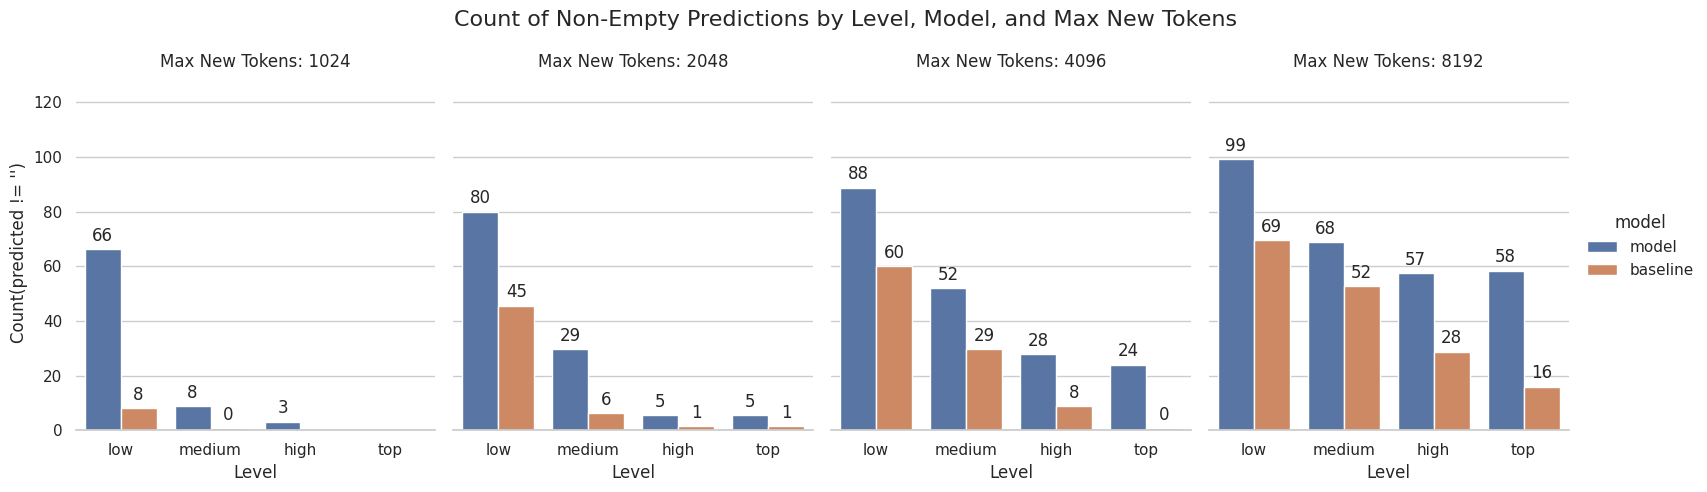
\includegraphics[width=0.9\linewidth]{model_comparison_plot_pct.png}
    \end{center}
    \begin{center}
        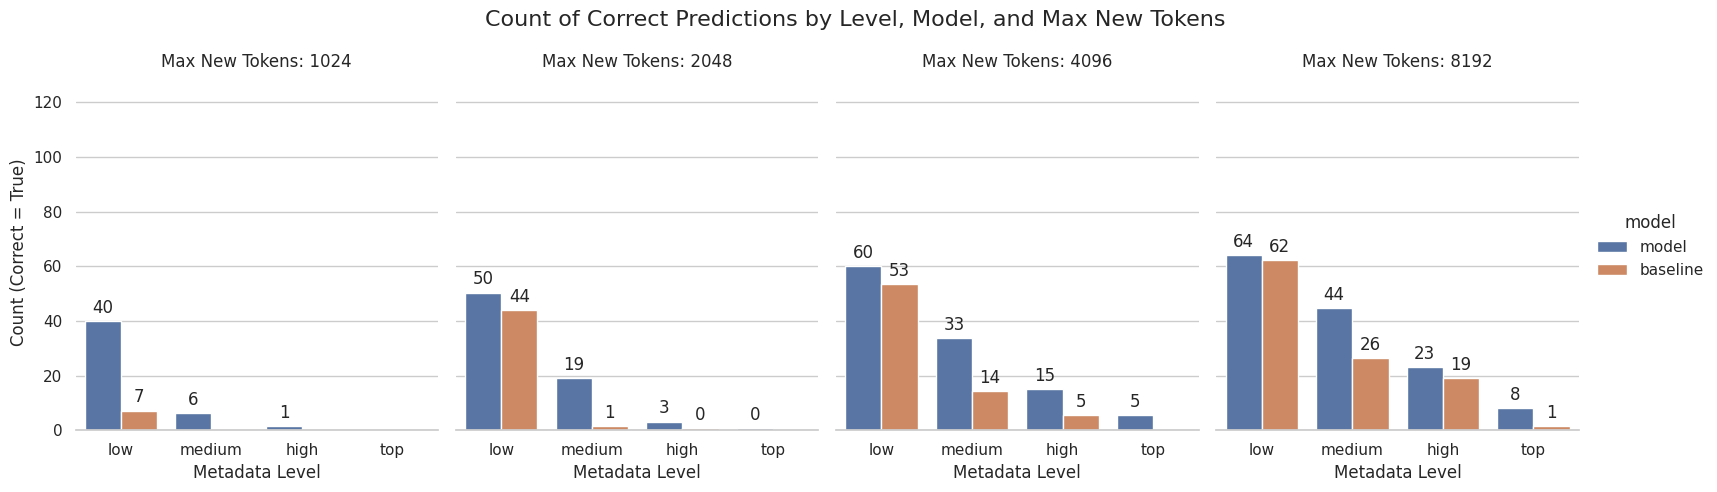
\includegraphics[width=0.9\linewidth]{correct_model_comparison_plot_pct.png}
    \end{center}
  \end{block}

  \begin{block}{Conclusion}

    Cognitive Compression is a powerful tool for efficient long-context modeling:
    \begin{itemize}
        \item Optimizes inference on hardware-constrained systems.
        \item Distinguishes between intermediate "thought" and terminal "solution" tokens.
        \item Enables graceful degradation rather than system failure.

    \end{itemize}

  \end{block}

  \begin{block}{References}

    \nocite{*}
    \footnotesize{\bibliographystyle{plain}\bibliography{poster}}

  \end{block}

\end{column}

\separatorcolumn
\end{columns}
\end{frame}

\end{document}
